\section{Spline\-Coordinate Class Reference}
\label{classSplineCoordinate}\index{SplineCoordinate@{SplineCoordinate}}
{\tt \#include $<$splinecoordinate.h$>$}

Inheritance diagram for Spline\-Coordinate::\begin{figure}[H]
\begin{center}
\leavevmode
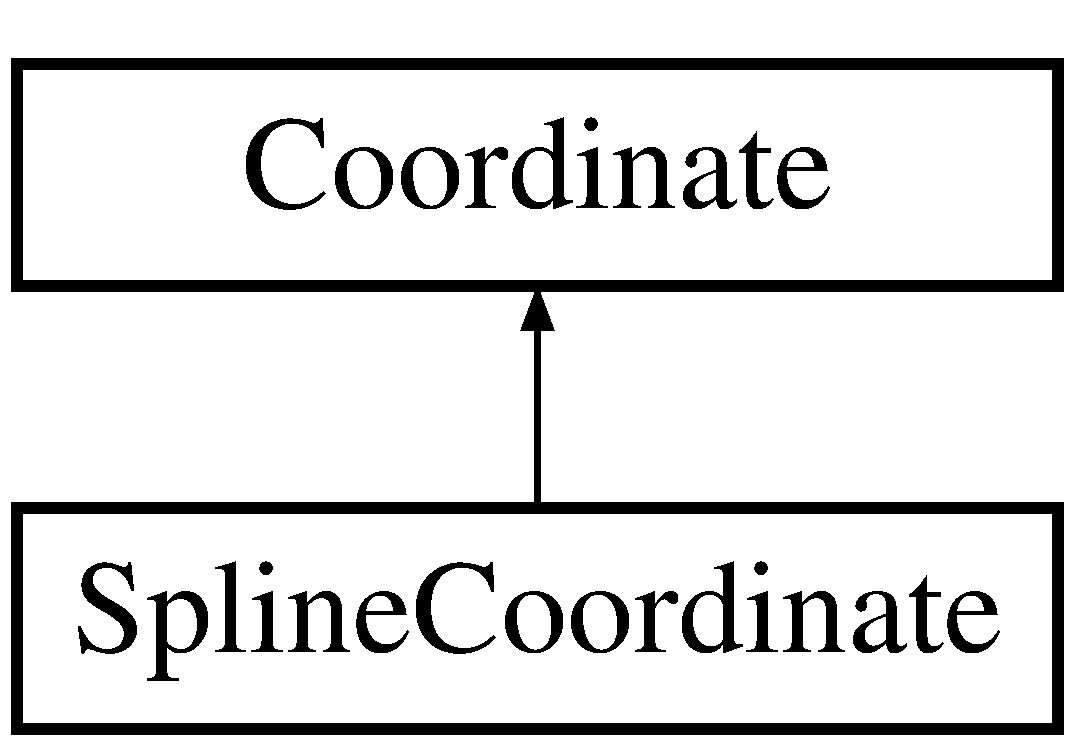
\includegraphics[height=2cm]{classSplineCoordinate}
\end{center}
\end{figure}
\subsection*{Public Methods}
\begin{CompactItemize}
\item 
{\bf Spline\-Coordinate} ()
\item 
{\bf Spline\-Coordinate} (int {\bf x}, int {\bf y}, float {\bf shape\-Factor})
\item 
{\bf Spline\-Coordinate} ({\bf Coordinate} $\ast$c, float shapefactor)
\item 
{\bf $\sim$Spline\-Coordinate} ()
\item 
void {\bf set\-Shape\-Factor} (float {\bf shape\-Factor})
\item 
float {\bf get\-Shape\-Factor} ()
\end{CompactItemize}
\subsection*{Private Attributes}
\begin{CompactItemize}
\item 
float {\bf shape\-Factor}
\end{CompactItemize}


\subsection{Detailed Description}
This class handles coordinates to be used in splines. This class is derived from {\bf Coordinate} {\rm (p.\,\pageref{classCoordinate})}. \begin{Desc}
\item[Author: ]\par
Anthony Liekens \end{Desc}




\subsection{Constructor \& Destructor Documentation}
\index{SplineCoordinate@{Spline\-Coordinate}!SplineCoordinate@{SplineCoordinate}}
\index{SplineCoordinate@{SplineCoordinate}!SplineCoordinate@{Spline\-Coordinate}}
\subsubsection{\setlength{\rightskip}{0pt plus 5cm}Spline\-Coordinate::Spline\-Coordinate ()}\label{classSplineCoordinate_a0}


Constructor. Constructs a spline coordinate. \index{SplineCoordinate@{Spline\-Coordinate}!SplineCoordinate@{SplineCoordinate}}
\index{SplineCoordinate@{SplineCoordinate}!SplineCoordinate@{Spline\-Coordinate}}
\subsubsection{\setlength{\rightskip}{0pt plus 5cm}Spline\-Coordinate::Spline\-Coordinate (int {\em x}, int {\em y}, float {\em shape\-Factor})}\label{classSplineCoordinate_a1}


Constructor. Constructs a spline coordinate. \begin{Desc}
\item[Parameters: ]\par
\begin{description}
\item[{\em 
x}]X-axis value of the coordinate \item[{\em 
y}]Y-axis value of the coordinate \item[{\em 
shape\-Factor}]The value of this factor must be between -1 (which means that the spline is interpolated at this point) and 1 (which means that the spline is approximated at this point). The spline is always smooth in the neighbourhood of a control point, except when the value of the factor is 0 for which there is a first-order discontinuity (i.e. angular point). \end{description}
\end{Desc}
\index{SplineCoordinate@{Spline\-Coordinate}!SplineCoordinate@{SplineCoordinate}}
\index{SplineCoordinate@{SplineCoordinate}!SplineCoordinate@{Spline\-Coordinate}}
\subsubsection{\setlength{\rightskip}{0pt plus 5cm}Spline\-Coordinate::Spline\-Coordinate ({\bf Coordinate} $\ast$ {\em c}, float {\em shapefactor})}\label{classSplineCoordinate_a2}


Constructor. Constructs a spline coordinate. \begin{Desc}
\item[Parameters: ]\par
\begin{description}
\item[{\em 
c}]{\bf Coordinate} {\rm (p.\,\pageref{classCoordinate})} of the spline coordinate \item[{\em 
shape\-Factor}]The value of this factor must be between -1 (which means that the spline is interpolated at this point) and 1 (which means that the spline is approximated at this point). The spline is always smooth in the neighbourhood of a control point, except when the value of the factor is 0 for which there is a first-order discontinuity (i.e. angular point). \end{description}
\end{Desc}
\index{SplineCoordinate@{Spline\-Coordinate}!~SplineCoordinate@{$\sim$SplineCoordinate}}
\index{~SplineCoordinate@{$\sim$SplineCoordinate}!SplineCoordinate@{Spline\-Coordinate}}
\subsubsection{\setlength{\rightskip}{0pt plus 5cm}Spline\-Coordinate::$\sim$Spline\-Coordinate ()}\label{classSplineCoordinate_a3}


Destructor. Destructs a spline coordinate. 

\subsection{Member Function Documentation}
\index{SplineCoordinate@{Spline\-Coordinate}!getShapeFactor@{getShapeFactor}}
\index{getShapeFactor@{getShapeFactor}!SplineCoordinate@{Spline\-Coordinate}}
\subsubsection{\setlength{\rightskip}{0pt plus 5cm}float Spline\-Coordinate::get\-Shape\-Factor ()\hspace{0.3cm}{\tt  [inline]}}\label{classSplineCoordinate_a5}


Returns the shape factor. \begin{Desc}
\item[Returns: ]\par
float \end{Desc}
\index{SplineCoordinate@{Spline\-Coordinate}!setShapeFactor@{setShapeFactor}}
\index{setShapeFactor@{setShapeFactor}!SplineCoordinate@{Spline\-Coordinate}}
\subsubsection{\setlength{\rightskip}{0pt plus 5cm}void Spline\-Coordinate::set\-Shape\-Factor (float {\em shape\-Factor})\hspace{0.3cm}{\tt  [inline]}}\label{classSplineCoordinate_a4}


Set the shape factor \begin{Desc}
\item[Parameters: ]\par
\begin{description}
\item[{\em 
shape\-Factor}]The value of this factor must be between -1 (which means that the spline is interpolated at this point) and 1 (which means that the spline is approximated at this point). The spline is always smooth in the neighbourhood of a control point, except when the value of the factor is 0 for which there is a first-order discontinuity (i.e. angular point). \end{description}
\end{Desc}
\begin{Desc}
\item[Returns: ]\par
void \end{Desc}


\subsection{Member Data Documentation}
\index{SplineCoordinate@{Spline\-Coordinate}!shapeFactor@{shapeFactor}}
\index{shapeFactor@{shapeFactor}!SplineCoordinate@{Spline\-Coordinate}}
\subsubsection{\setlength{\rightskip}{0pt plus 5cm}float Spline\-Coordinate::shape\-Factor\hspace{0.3cm}{\tt  [private]}}\label{classSplineCoordinate_o0}




The documentation for this class was generated from the following files:\begin{CompactItemize}
\item 
{\bf splinecoordinate.h}\item 
{\bf splinecoordinate.cpp}\end{CompactItemize}
